
\everymath{\displaystyle}  

\chapter{Cơ Sở Lý Thuyết}
\label{chap:chap3}

\noindent Trong chương này tôi sẽ trình bày về một số lý thuyết cơ bản để tiếp cận với mạng nerual dễ dàng hơn. 

\section{Các khái niệm cơ bản}
\begin{itemize}
	\item \textbf{Quan sát}: kí hiệu là \textbf{x}, input trong các bài toán. Quan sát thường có dạng là một vector $\textbf{x}=(x_1,x_2,x_3,\ldots, x_n)$, gọi là \textbf{feature vector}. Mỗi $x_i$ gọi là một feature. Ví dụ bạn muốn đoán xem hôm nay có mưa không dựa vào observation gồm các feature (nhiệt độ, độ ẩm, tốc độ gió).	
\item \textbf{Label}: kí hiệu là $y$, output của bài toán. Mỗi quan sát sẽ có một label tương ứng. Ở ví dụ về mưa ở trên label chỉ là "mưa" hoặc "không mưa"; hay về điểm thì là các số thực từ 0 đến 10. Label có thể mang nhiều dạng nhưng đều có thể chuyển đổi thành một số thực hoặc một vector. 
\item \textbf{Model}: trong chương này các bạn hiểu là nó là một hàm số $f(x)$, nhận vào một đầu vào \textbf{x} và trả về một đầu ra dự đoán (predict) $y=f(\textbf{x})$.
\item \textbf{Parameter}: mọi thứ của model được sử dụng để tính toán ra output. Ví dụ model là một hàm đa thức bậc hai: $f(x) = ax_1^2 + bx_2 + c$ thì parameter của nó là bộ ba $(a,b,c)$. Để ngắn gọn, người ta thường gom tất cả parameter của một model lại thành một vector, thường được kí hiệu là $\textbf{w}$ và biểu diễn thông qua hàm $f(\textbf{x},\textbf{w}) = \textbf{x}\textbf{w}$.

\end{itemize}
\section{Huấn luyện mạng}
Một mạng nơron được huyấn luyện sao cho với một tập các vector đầu vào
X, mạng có khả năng tạo ra tập các vector đầu ra mong muốn Y của nó. Tập \textbf{X} được sử dụng cho huấn luyện mạng được gọi là tập huấn luyện (training set). Các phần tử \textbf{x} thuộc \textbf{X} được gọi là các mẫu huấn luyện (training example). Quá trình huấn luyện bản chất là sự thay đổi các trọng số liên kết của mạng. Trong quá trình này, các trọng số của mạng sẽ hội tụ dần tới các giá trị sao cho với mỗi vector đầu vào \textbf{x} từ tập huấn luyện, mạng sẽ cho ra vector đầu ra y như mong muốn.\par
Có hai phương pháp học phổ biến là học có giám sát (supervised learning), học không giám sát (unsupervised learning):

\begin{itemize}
	\item \textbf{Học có giám sát}: Là quá trình học có sự tham gia giám sát của một "thầy giáo". Giống như ta dạy trẻ nhận diện các loại phương tiện. Ta đưa ra hình ô tô và bảo với trẻ đó rằng đây là chiếc ô tô. Việc này được thực hiện trên các loại phương tiện khác nhau như xe máy, máy bay, xe đạp.... Sau đó khi kiểm tra ta sẽ đưa ra một hình phương tiện bất kì, các hình này hơi khác so với các hình đã dạy trẻ, và cho trẻ đoán xem xe này thuộc loại phương tiện nào?\\
	Như vậy với học có giám sát, số lớp cần phân loại đã được biết trước. Nhiệm vụ của thuật toán là phải xác định được một cách thức phân lớp sao cho với mỗi vector đầu vào sẽ được phân loại chính xác vào lớp của nó
	
	\item \textbf{Học không giám sát}: Là việc học không cần có bất kỳ một sự giám sát nào.Trong bài toán học không giám sát, chúng ta không biết câu trả lời chính xác cho mỗi dữ liệu đầu vào. Nhiệm vụ của thuật toán là phải phân chia tập dữ liệu đầu vào thành các nhóm con, mỗi nhóm chứa các đặc trưng giống nhau. Ví dụ như phân nhóm loại khách hàng dựa trên hành vi mua hàng: số lượng hàng hóa mua, loại hàng hóa mua, khoảng thời gian cách nhau giữa mỗi lần mua,....\\
	 Như vậy với học không giám sát, số lớp phân loại chưa được biết trước, và tùy theo tiêu chuẩn đánh giá độ tương tự giữa các mẫu mà ta có thể có các lớp phân loại khác nhau.

\end{itemize}
Tài liệu này tôi sẽ trình bày về phần học có giám sát thông qua mạng nơ-ron nhân tạo và mạng tích chập.

\section{Định nghĩa}
Mạng nơron nhân tạo, Artificial Neural Network (ANN) là một mô hình xử lý thông tin phỏng theo cách thức xử lý thông tin của các hệ nơ-ron sinh học. Nó được tạo nên từ một số lượng lớn các phần tử (nơ-ron) kết nối với nhau thông qua các liên kết (trọng số liên kết) làm việc như một thể thống nhất để giải quyết một vấn đề cụ thể nào đó. Một mạng nơ-ron nhân tạo được cấu hình cho một ứng dụng cụ thể (nhận dạng mẫu, phân loại dữ liệu,...) thông qua một quá trình học từ tập các mẫu huấn luyện. Về bản chất học chính là quá trình hiệu chỉnh trọng số liên kết giữa các nơ-ron.

\section{Cấu tạo của một nơ-ron}
\label{sec:neuralStruct}
Trong phần này tôi sẽ trình bày chi tiết cấu trúc của một nơ-ron \ref{fig:aNeural} trong mạng lưới nơ-ron.
\begin{center}
    \begin{figure}[h]
    \begin{center}
     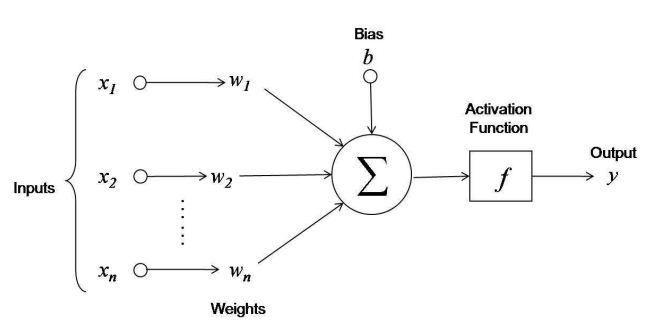
\includegraphics[scale=0.5]{chap3/image/cauTrucMotNoron.jpg}
    \end{center}
    \caption{Cấu trúc của một nơ-ron}
 	\label{fig:aNeural}
    \end{figure}
\end{center}
\par
 Các thành phần cơ bản của nơ-ron:

\begin{enumerate}
\setlength{\itemindent}{5mm}
	\item \textbf{Đầu vào} (\textbf{x}): các tín hiệu vào của nơ-ron, các tín hiệu này thường đưa vào dưới dạng một vector N chiều và được kí hiệu là $\textbf{x}$ và mỗi phần tử trong vector được kí hiệu là $x_i, i\in{0,n}$
	\item \textbf{Trọng số} (\textbf{w}): mỗi liên kết được thể hiện bởi một trọng số liên kết và được gọi là weight. Trọng số liên kết giữa tín hiệu vào thứ j với nơ-ron k thường được kí hiệu là $w_{kj}$, và. Thông thường, các trọng số này được khởi tạo một cách ngẫu nhiên theo phân phối chuẩn ở thời điểm khởi tạo mạng và được cập nhật liên tục trong quá trình học mạng.

	\item \textbf{Bias} (b): là tham số nhằm tăng khả năng thích ứng của mạng nơron trong quá trình học. Bias gần giống như trọng số, trừ một điều là nó luôn có tín hiệu vào không đổi bằng 1 (được trình bày rõ hơn ở phần \ref{subsec:feedforward} ). Tham số này có thể bỏ đi nếu không cần thiết.	
	
	\item \textbf{Hàm kết hợp} (z): Mỗi một đơn vị trong một mạng kết hợp các giá trị đưa vào nó thông qua các liên kết với các đơn vị khác, sinh ra một giá trị gọi là net input. Hàm thực hiện nhiệm vụ này  gọi là hàm kết hợp (combination function), được định nghĩa bởi một luật lan truyền cụ thể. Thông thường hàm này sẽ là hàm tổng của tích các trọng số với đầu vào và độ lệch. Và được biể diễn thông qua biểu thức $z = \sum_{i=1}^n(x_iw_i) +b$.
	\item \textbf{Hàm truyền (activiation function hoặc transfer function)}: Hàm này được dùng để giới hạn phạm vi đầu ra của mỗi nơ-ron và nhận đầu vào là kết quả của hàm kết hợp. Tôi sẽ trình bày phần này rõ hơn ở phần \ref{sec:activationFunc}.
	\item \textbf{Đầu ra (output)}: Là tín hiệu đầu ra của một nơ-ron, với mỗi nơ-ron sẽ có tối đa là một đầu ra. Nếu như nơ-ron đó ở các hidden layer thì đầu ra của nó được gọi là activation và được kí hiệu là $a$.
\end{enumerate} \par
Khi quy về toán học thì một nơ-ron sẽ được thể hiện thông qua hai hàm sau:
\begin{center}
$z = \sum_{i=1}^n(x_iw_i)+b = \textbf{x}\textbf{w}+b$\\[5pt]
$a = f(z)$
\end{center}
\par
Trong đó:
\begin{itemize}
\setlength{\itemindent}{5mm}
	\item[\textendash] $x_i,w_i$ là giá trị thứ $i$ của đầu vào và trọng số tương ứng
	\item[\textendash] Hàm $f$ là hàm truyền và có đầu vào là giá trị của bộ tổng $z$
	\item[\textendash] $a$ là giá trị được tính bởi hàm truyền và là đầu ra của nơ-ron
\end{itemize}
\par
Như vậy một nơ-ron nhận các đầu vào sau đó kết hợp với các trọng số rồi đưa kết quả vào hàm truyền và cho ra một giá trị đầu ra.

\section{Cấu trúc của mạng nơ-ron}

\subsection{Layer}
Mạng neural  được chia làm 3 lớp chính: lớp đầu vào (\textit{input layer}, màu vàng), lớp ẩn (\textit{hidden layer}, màu xanh lá), lớp đầu ra (\textit{output layer}, màu xanh dương) và trong mỗi lớp có số lượng \textit{unit} khác nhau. Cấu trúc mạng được minh họa trong Hình \ref{fig:neuralNetworkStruct}.
\begin{center}
 	\begin{figure}[htp]
    \begin{center}
     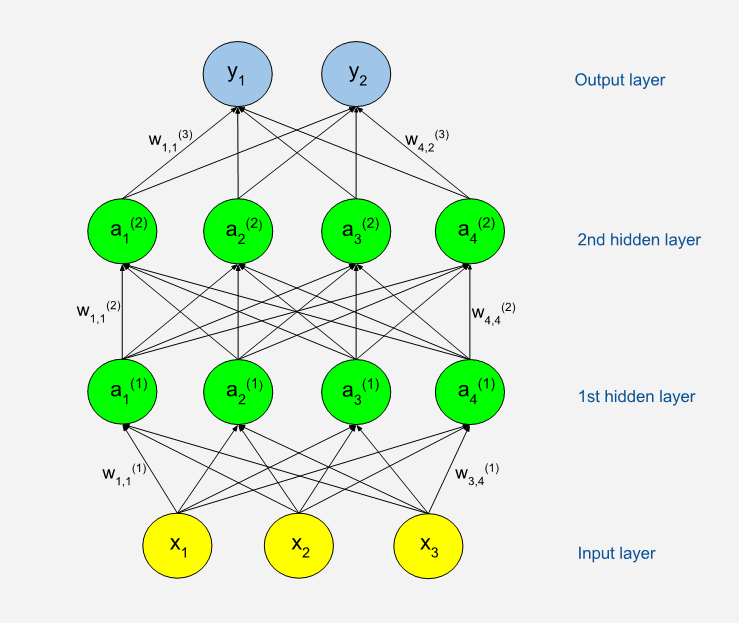
\includegraphics[scale=0.5]{chap3/image/cautrucNN.png}
    \end{center}
    \caption{Cấu trúc mạng nơ-ron}
    \label{fig:neuralNetworkStruct}
    \end{figure}
\end{center}

\begin{itemize}
\setlength{\itemindent}{5mm}
	\item \textit{Input layer}: Biểu diễn tổng quát của mỗi quan sát
	\item \textit{Output layer}: Thể hiện đầu ra dự đoán của model
	\item \textit{Hidden layer}: Là lớp thể hiện cấu trúc của mạng nơ-ron. Các \textit{hidden layer} theo thứ tự từ input layer đến output layer được đánh số thứ tự là \textit{hidden layer 1, hidden layer 2,...}.
\end{itemize}\par
Số lượng layer trong một mạng nơ-ron được ký hiệu là $L$ và được tính bằng số hidden layer cộng thêm một. Ví dụ trong Hình \ref{fig:neuralNetworkStruct}, $L=3$.
\subsection{Units}
Mỗi \textit{node} hình trong trong Hình \ref{fig:neuralNetworkStruct} được gọi là một \textit{unit} hoặc một nơ-ron. Như tôi đã trình bày cấu trúc của một nơ-ron ở phần \ref{sec:neuralStruct}, đầu vào của một nơ-ron là một hàm kết hợp và đầu ra thông qua một hàm gọi là activiation. Ở mạng nơ-ron thì đầu vào của hidden layer thứ $l$ được ký hiệu là $\textbf{z}^{(l)}$ với $z^{(l)}_i = \textbf{x}\textbf{w}^{(l)}_i$ và đầu ra của mỗi unit được ký hiệu là $\textbf{a}^{(l)}$ với $\textbf{a}^{(l)}= f(\textbf{z}^{(l)})$.\par

	Số lượng unit trong mỗi lớp, số lượng lớp trong mỗi cấu trúc mạng là không xác định. Nó được xây dựng dựa vào kinh nghiệm của người thiết kế mạng hoặc theo các tài liệu đã được công bố. Nếu số lượng lớp quá lớn thì tốc độ tính toán chậm, còn số lượng lớp ít thì độ tin cậy của kết quả không cao. Nếu số node trong các lớp lớn thì sẽ bị overfitting, ngược lại sẽ bị underfitting. Tôi sẽ trình bày phần overfitting, underfitting ở phần sau.
\section{Hàm truyền (activation function)}
\label{sec:activationFunc}
Phần lớn các đơn vị trong mạng nơron chuyển net input  bằng cách sử dụng một hàm vô hướng (scalar-to-scalar function) gọi là hàm kích hoạt, kết quả của hàm này là một giá trị gọi là mức độ kích hoạt của đơn vị (unit's activation). Loại trừ khả năng đơn vị đó thuộc lớp ra, giá trị kích hoạt được đưa vào một hay nhiều đơn vị khác. Các hàm kích hoạt thường bị ép vào một khoảng giá trị xác định, do đó thường được gọi là các hàm bẹp (squashing). Một số hàm thường được sử dụng là ReLU, sigmoid, softmax.\par
	\subsection{Hàm ReLU}
	\label{sec:relu}
	Hàm ReLU (Rectified Linear Unit) được sử dụng rộng rãi gần đây vì tính đơn giản của nó. Nó có công thức toán học  $f(s)=\max(0,s)$. Đồ thị hàm ReLU được thể hiện ở Hình \ref{fig:relu}
\begin{center}
 	\begin{figure}[htp]
    \begin{center}
    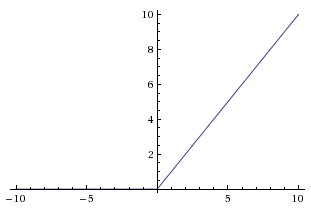
\includegraphics[scale=1]{chap3/image/relu.jpeg}
    \end{center}
    \caption{Hàm ReLU}
    \label{fig:relu}
    \end{figure}
\end{center}
	Từ biểu đồ ta có thể dễ dàng thấy độ lệch của hàm ReLU luôn bằng 1 khi $x>0$, bằng 0 khi $x<0$ và ta quy ước tại  $x=0$ thì độ lệch bằng 0 nhưng trường hợp này rất ít khi xảy ra.\\
	
\begin{center}
	$\frac{d}{dx}ReLU(x) =
    \begin{cases}
       0,$ if $x < 0,\\
       1,  otherwise.
    \end{cases}
    $
\end{center}
	Hàm ReLU thường được sử dụng làm hàm truyền trong các hidden layer, còn ở layer cuối cùng thì ta sẽ sử dụng hàm khác để có thể tính toán được sắc xuất dự đoán vào vùng phân loại.

\subsection{ Hàm sigmoid}
	 Hàm logistic là mô hình một dạng đường cong-S của sự tăng trưởng của một tập $P$ nào đó. Sự tăng trưởng được mô hình như sau: giai đoạn tăng trưởng ban đầu được xấp xỉ hàm mũ và khi quá trình bão hòa bắt đầu, sự phát triển sẽ chậm lại, và tới giai đoạn trưởng thành thì dừng hẳn. \par 
	 Hàm logistic có công thức toán học là: 
	 \begin{center}
	 	$P(x,a,m,n,r) = a\frac{1+m\exp({-x/r})}{1+n\exp({-x/r})}$ \rule{5mm}{0pt} với $a,m,n,r$ là các tham số thực.
	 \end{center}
	 \par
	  Hàm sigmoid là một trường hợp đặc biệt của hàm logistic và có công thức toán học là $\sigma(x) = \frac{1}{1+\exp({-t})}$, đồ thị được thể hiện ở Hình \ref{fig:sigmoid}
\begin{center}
 	\begin{figure}[htp]
    \begin{center}
    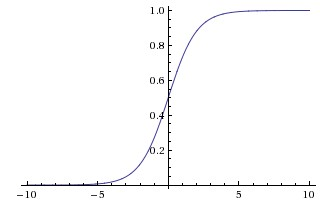
\includegraphics[scale=1]{chap3/image/sigmoid.jpeg}
    \end{center}
    \caption{Hàm sigmoid}
    \label{fig:sigmoid}
    \end{figure}
\end{center}
Nhìn vào đồ thị ta có thể thấy giá trị của hàm nằm trong khoảng (0,1]. Cụ thể, với đầu vào lớn hàm số sẽ cho đầu ra gần với 1 còn với đầu vào nhỏ hàm số sẽ cho đầu ra gần với 0. Hàm số này được sử dụng nhiều trong quá khứ vì có đạo hàm $\frac{d\sigma(x)}{d(x)} = \sigma(x).(1-\sigma(x)$ rất đẹp. Những năm gần đây, hàm số này ít khi được sử dụng do khi có đầu vào là những số cực lớn hoặc cực bé thì đạo hàm của hàm số xấp xỉ bằng 0, điều này gây ảnh hưởng đến việc cập nhập các trọng số trong quá trình học và làm cho thời gian tính toán lâu hơn. Tôi sẽ trình bày tại sao lại như vậy ở phần backpropagation.
	
	\subsection{Hàm softmax}
	\label{sec:softmax}
	Hàm softmax hay hàm trung bình mũ là sự khái quát hóa của hàm logistic biến không gian K-chiều véc tơ  với giá trị thực bất kỳ đến không gian K-chiều véc tơ  mang giá trị trong phạm vi (0, 1).\par

Hàm softmax có phương trình toán học như sau:
\begin{center}
	$y_i=\frac{\exp({x_i})}{\sum^{n}_{j=1}{\exp({x_j})}}; \forall i=1,...,n$ %\rule{5mm}{0pt} %
	
	
\end{center}	
với $n$ là số lượng phần tử trong vector \textbf{x}.\par
Hiện nay hàm này được sử dụng rộng rãi trong việc phân loại trong lớp đầu ra. Vì nếu tại giá trị phần tử $x_i$ lớn vượt trội so với toàn bộ dữ liệu ở vector $\textbf{x}$ thì giá trị đầu ra $y_i$ cũng sẽ lớn vượt trội so với đầu ra ở các phần tử khác. Điều tiếp theo chúng ta có thể thấy rằng tổng đầu ra sẽ luôn bằng môt, softmax đã sử dụng hàm $\exp(x)=e^{x}$ (Hình \ref{fig:hamex}) giúp cho giá trị của đầu ra luôn dương và thứ tự các phần tử đầu ra tương ứng với thứ tự đầu vào.
\begin{center}
	\begin{figure}[htp]
	\begin{center}
		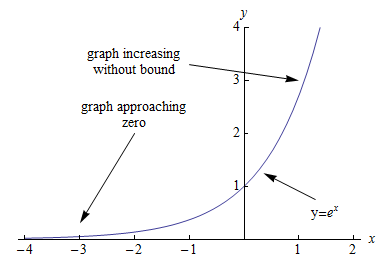
\includegraphics[scale=1]{chap3/image/expgraph.png}
	\end{center}			
	\caption{Đồ thị hàm $f(x)=\exp(x)$}
	\label{fig:hamex}
	\end{figure}
\end{center}

Một vài ví dụ về hàm softmax, với dữ liệu đầu vào là vector \textbf{z} và giá trị đầu ra là vector \textbf{a}, giá trị các vector được thể hiện qua Hình \ref{fig:vdsoftmax}.
\begin{center}
	\begin{figure}[htp]
	\begin{center}
		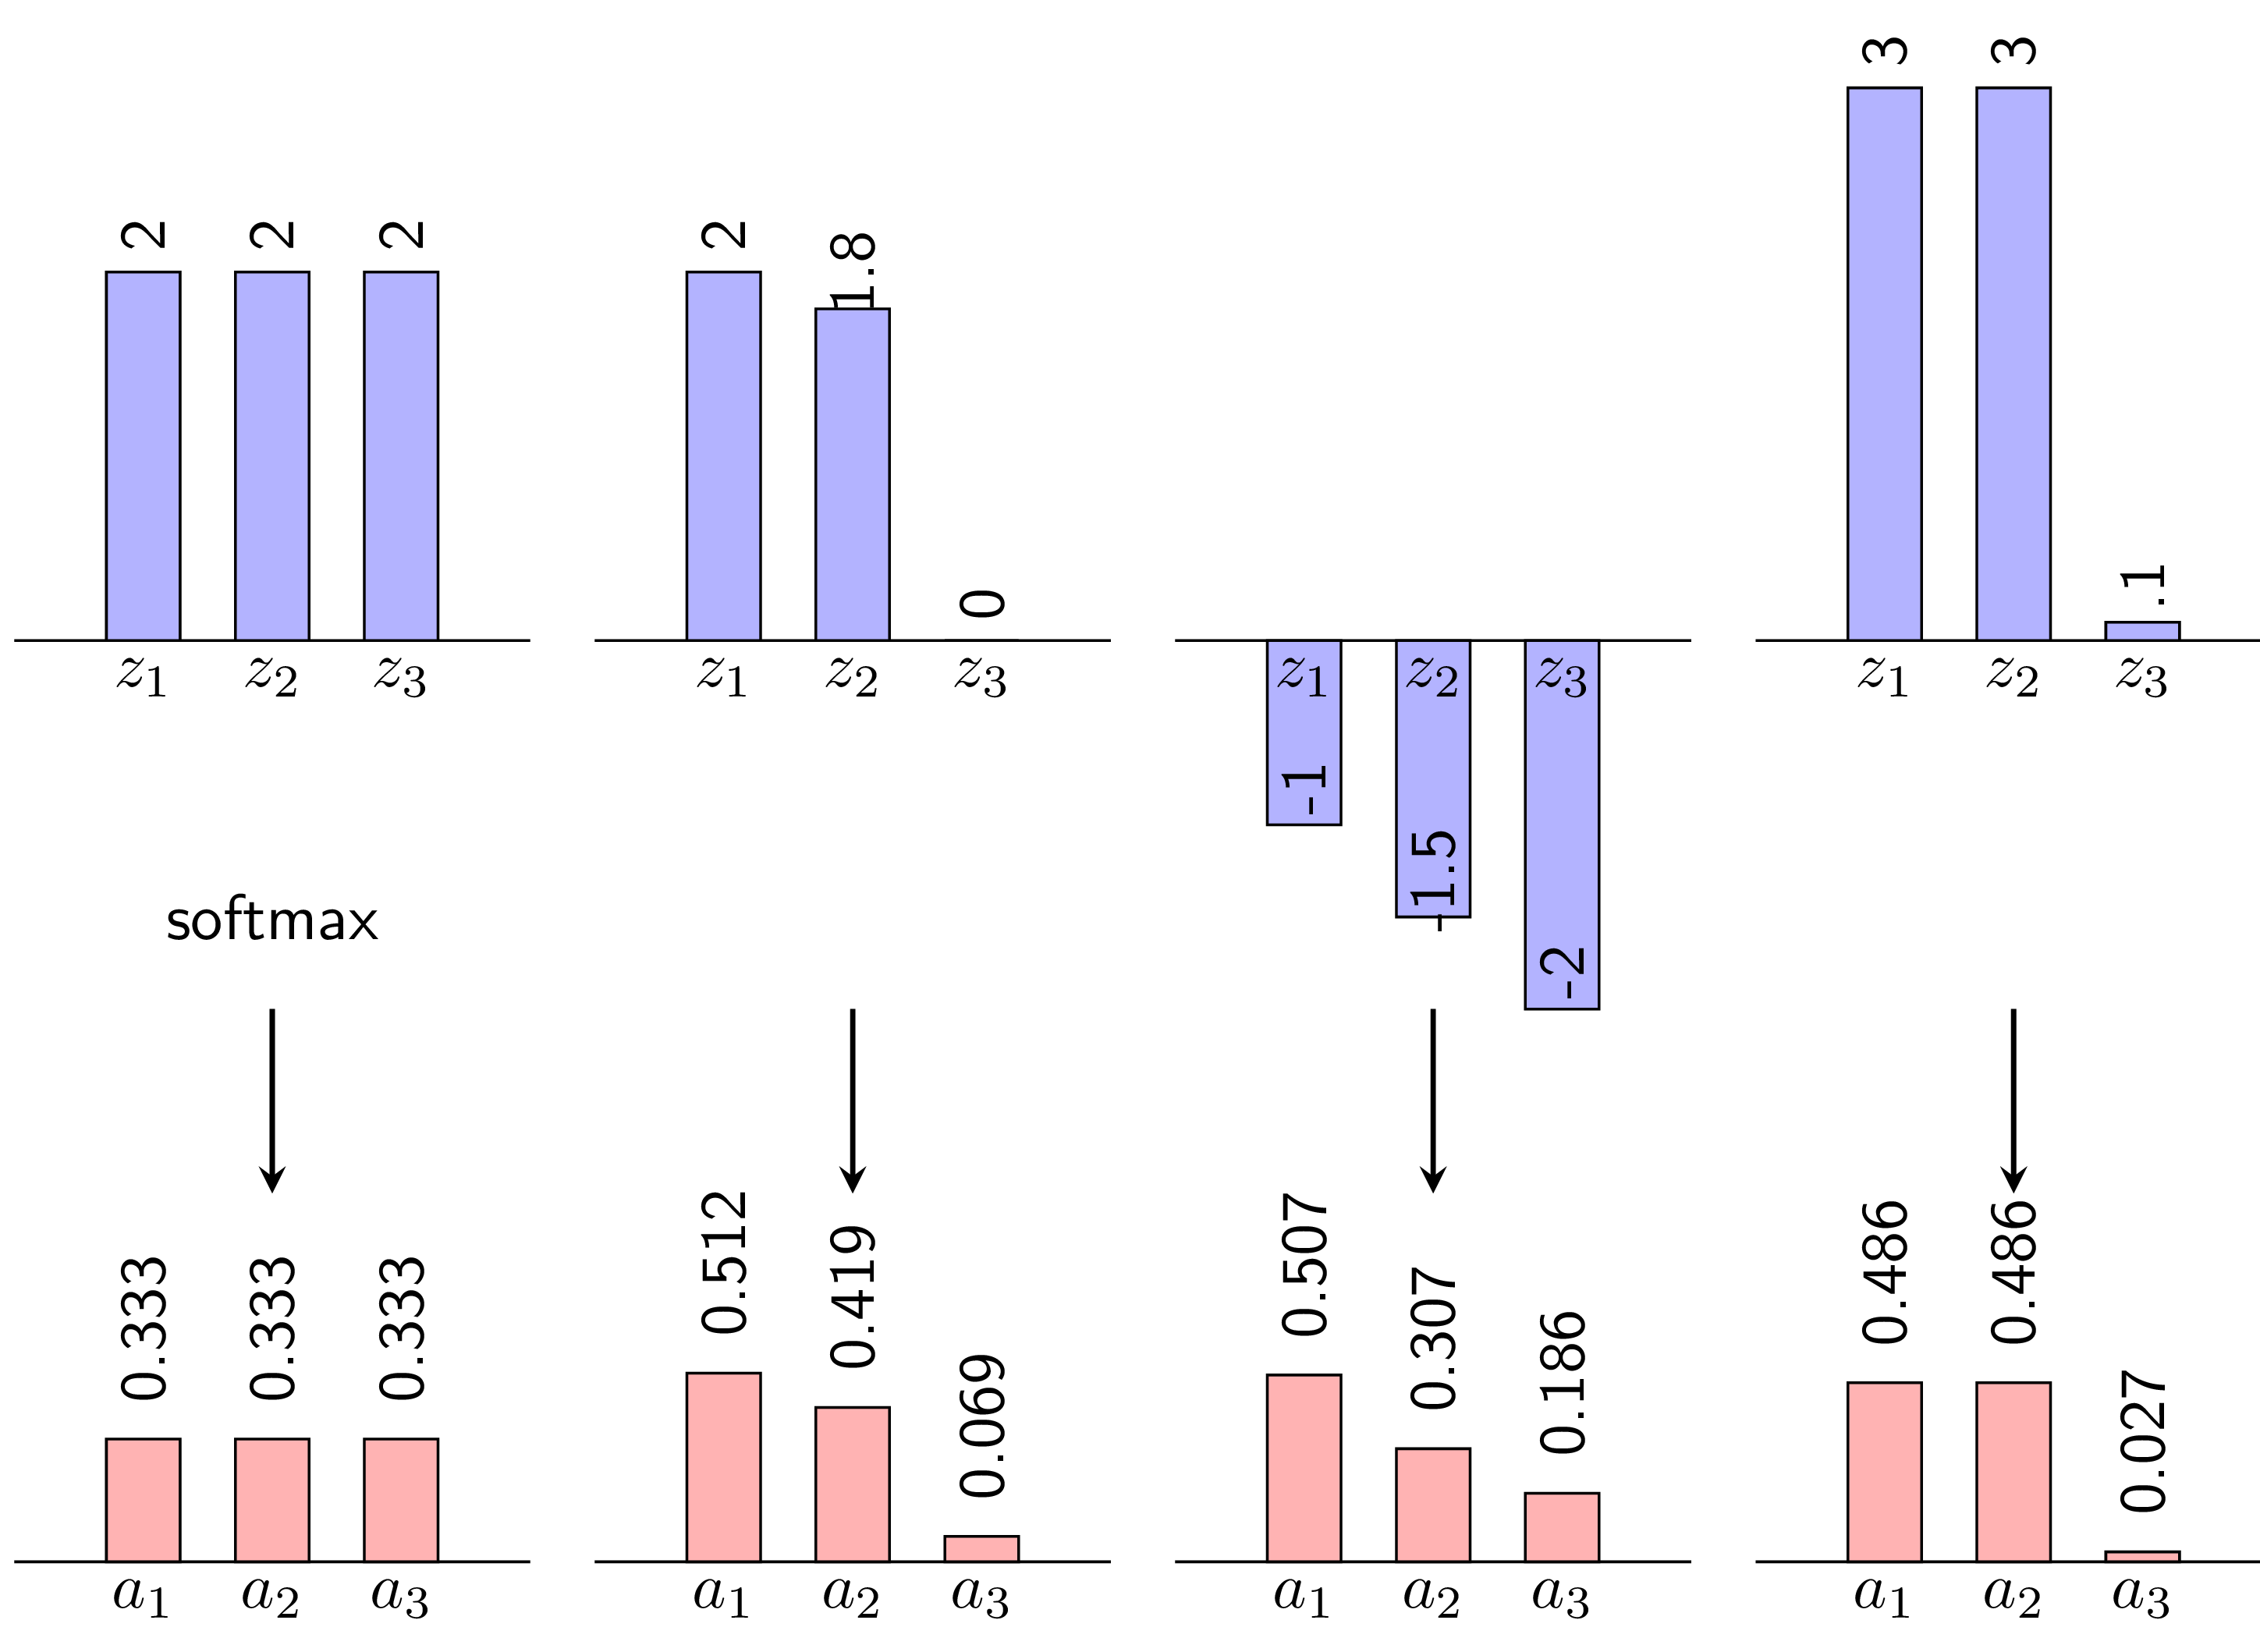
\includegraphics[scale=0.1]{chap3/image/softmax_ex.png}
	\end{center}			
	\caption{Ví dụ hàm softmax}
	\label{fig:vdsoftmax}
	\end{figure}
\end{center}
Tại đây chúng ta có thể thấy giá trị của đầu ra luôn dương, giá trị đầu ra lớn nhất tại giá trị ở phần tử đầu vào lớn nhất, tổng các giá trị đầu ra luông bằng 1. \par

Như vậy với hàm softmax chúng ta có với mỗi đầu ra \textit{$y_i$} luôn phụ thuộc vào tất cả \textit{$x_i$} và đầu ra luôn dương, tổng đầu ra bằng một, thứ tự đầu vào tương ứng với đầu ra. Vì thế  đầu ra $y_i$ có thể coi là xắc suất để đầu vào $x_i$ rơi vào lớp thứ $i$.



\section{Mạng lan truyền thẳng}
\label{sec:forward}
%\subsection{Truyền thẳng}
%Truyền thẳng là ta tính giá trị đầu ra thông qua các đầu vào cho trước theo thứ tự tính toán trong toán học. 
%Để rõ ràng hơn tôi sẽ trình bày thông qua một ví dụ đơn giản.\par
%Giả sử chúng ta cần tính giá trị hàm  $f(x,y,z) = (x+y)*z$ với $x=-2,y=5,z=-4.$
%Với dữ liệu trên thì ta có thể tính toán đơn giản thông qua phép cộng, nhân và theo thứ tự là trong ngoặc trước, ngoài ngoặc sau. Chúng ta sẽ xây dựng biểu thức trên  một đồ thị với đỉnh là các toán tử (cộng, trừ, nhân, chia, mũ, logarit ...) và lá là các phần tử tham gia đến việc tính toán của đỉnh, đồ thị được thể hiện thông qua Hình \ref{fig:dothi}.
%\begin{center}
%    \begin{figure}[H]
%    \begin{center}
%     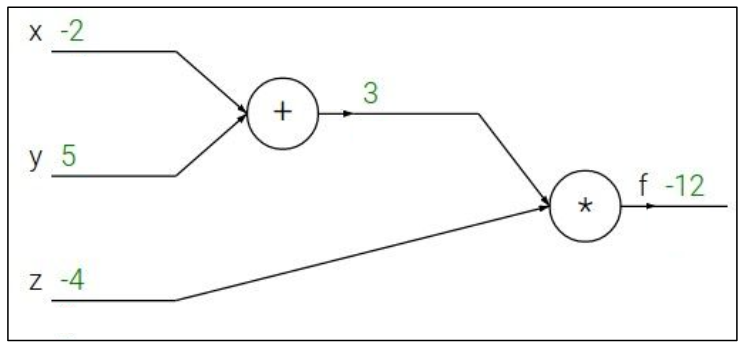
\includegraphics[scale=1]{chap3/image/graph_fw_bp.png}
%    \end{center}
%    \caption{Đồ thị tính toán}
%    \label{fig:dothi}
%    \end{figure}
%\end{center}
%
%Chúng ta sẽ tính hàm $f(x,y,z)$ theo thứ tự của đồ thị. Giả sử ta đặt $q$ là tổng của $x,y$, như vậy để tính được giá trị của hàm $f$ ta cần tính giá trị của tổng $q$ sau đó nhân với giá trị của $z$.
%\begin{enumerate}
%	\item Tính tổng q $q= x+y = -2+5 =3$
%	\item Giá trị của hàm $f=q*z=3*4=12$
%\end{enumerate}
%Với cách tính trên ta gọi đó là truyền thẳng vì nó tính lần lượt và theo thứ tự xác định.
%\subsection{Lan Truyền thẳng trong mạng neural}
\subsection{Ví dụ}
Giả sử ta có mạng neural như Hình \ref{fig:baitoan} với tập dữ liệu đầu vào là ma trận $\textbf{X}_{2{\times}N}$ ($N$ là số lượng quan sát, 2 là số lượng feature), và label tương ứng là vector $\textbf{y}_{N\times 1}$ (2 là số lượng nhãn), $\textbf{y}_i \in (1,2,3,\ldots,C)$ với C là số lớp cần phân loại .

\begin{figure}[H]
\begin{center}
	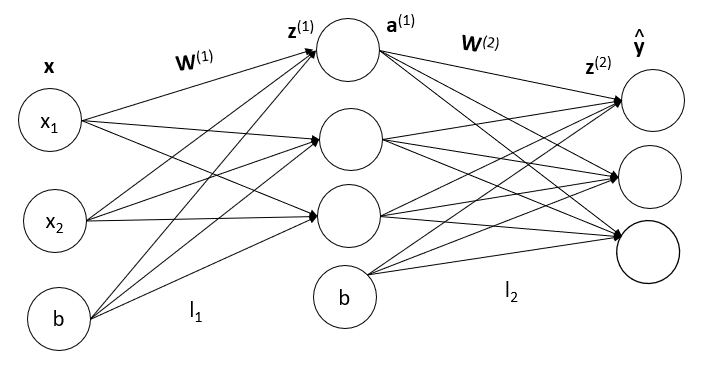
\includegraphics[scale=1]{chap3/image/myNeuralNetwork.png}
	\caption{Mạng neural cho bài toán }
	\label{fig:baitoan}
\end{center}
\end{figure}


Xét một cặp dữ liệu $(\textbf{x}_i,\textbf{y}_i)$ với hàm activation ở hidden layer là hàm relu, hàm activation ở output layer là hàm softmax. Mạng lan truyền thẳng sẽ được tính như sau:

\begin{equation}
\label{eq:s1}
\begin{aligned}
\textbf{x}_{1\times 2}& = \begin{bmatrix}
x_1 &x_2
\end{bmatrix}&
\textbf{W}^{(1)T}_{3{\times}2} &	=  \begin{bmatrix}
	w^{(1)}_{11} &w^{(1)}_{12} \\[6pt]
	w^{(1)}_{21} &w^{(1)}_{22} \\[6pt]
	w^{(1)}_{31} &w^{(1)}_{32} 
\end{bmatrix}^{T}
\end{aligned}
\end{equation}

	\begin{equation}
	\label{eq:s2}
	\begin{aligned}		
	\textbf{z}^{(1)}_{1 \times 3}	&	=\textbf{x}_{1\times 2}\textbf{W}^{(1)T}_{3\times 2} +b^{(1)}\\
%	&	=\begin{bmatrix}
%	w^{(1)}_{11}x_1+w^{(1)}_{12}x_2+b^{(1)} &w^{(1)}_{21}x_1 + w^{(1)}_{22}x_2+b^{(1)} & w^{(1)}_{31}x_1+w^{(1)}_{32}x_2+b^{(1)}
%	\end{bmatrix}\\
	&	=\begin{bmatrix}
	z^{(1)}_{1} &z^{(1)}_{2} &z^{(1)}_{3} 
	\end{bmatrix}		
	\end{aligned}
	\end{equation}


%Vì sử dụng hàm relu $f(s)=\max(0,s)$ cho hàm activation nên ta có: \par
\begin{equation}
\label{eq:s3}
\begin{split}
\textbf{a}^{(1)}_{1 \times 3}	&	=\max(0,\textbf{z}^{(1)})\\
	&	 = \begin{bmatrix}
	a^{(1)}_1 &a^{(1)}_2 &a^{(1)}_3 
	\end{bmatrix}
\end{split}
\end{equation}
\begin{equation}
\label{eq:s4}
\textbf{W}^{(2)T}_{3{\times}3} = \begin{bmatrix}
	w^{(2)}_{11} &w^{(2)}_{11} & w^{(2)}_{13}\\[6pt]
	w^{(2)}_{21} &w^{(2)}_{22} & w^{(2)}_{23}\\[6pt]
	w^{(2)}_{31} &w^{(2)}_{32} & w^{(2)}_{33}
\end{bmatrix}^T\\
\end{equation}
\begin{equation}
\label{eq:s5}
\begin{split}
\textbf{z}^{(2)}_{1\times 3}	&	=\textbf{a}^{(1)}_{1 \times 3}\textbf{W}^{(2)T}_{3{{\times}}3}+b^{(2)}\\
&	 = \begin{bmatrix}
z^{(2)}_{1} &z^{(2)}_{2} &z^{(2)}_{3} 
\end{bmatrix}
\end{split}
\end{equation}

\begin{equation}
\label{eq:s6}
\textbf{a}^{(2)}_{1\times 3} = \frac{\exp({\textbf{z}^{(2)}})}{\sum^{2}_{j=1}{\exp({\textbf{z}^{(3)}_j})}}
\end{equation}
\begin{equation*}
\widehat{\textbf{y}}=\textbf{a}^{(2)}_{1\times 3}
\end{equation*}

Tại các biểu thức số \ref{eq:s1},\ref{eq:s4} là giá trị đầu vào và khởi tạo ma trận trọng số cho layer thứ 1,2; tại biểu thức số \ref{eq:s2},\ref{eq:s5} ta tính giá trị hàm kết hợp (bộ tổng) làm input đầu vào cho nơ-ron; tại biểu thức số \ref{eq:s3},\ref{eq:s6} ta tính đầu ra cho mỗi nơ-ron. Ở layer thứ nhất đầu ra nơ-ron sử dụng \textit{hàm ReLU} \ref{fig:relu} làm hàm activation vì thế tại biểu thứ số \ref{eq:s3} ta có  $\textbf{a}^{(1)}_{1 \times 3}	=\max(0,\textbf{z}^{(1)})$ còn tại layer thứ hai sử dụng \textit{hàm softmax} \ref{sec:softmax} làm hàm đầu ra cho nơ-ron nên ta có $\textbf{a}^{(2)}_{1\times 3} = \frac{\exp({\textbf{z}^{(2)}})}{\sum^{3}_{j=1}{\exp({\textbf{z}^{(2)}_j})}}$.


Với tập dữ liệu $(\textbf{X},\textbf{y} )$ thì ta có đầu ra dự đoán như sau:  
\begin{center}

	$\widehat{\textbf{Y}} =\frac{\exp({\textbf{z}^{(2)}_i})}{\sum^{2}_{j=1}{\exp({\textbf{z}^{(2)}_{ij}})}}$; với $i=1,2,...,N$ 

\end{center}
Việc tính toán tuần tự như vậy được được gọi là \textit{feedforward}.
\subsection{ Thuật toán}
\label{subsec:feedforward}
Nếu ta thêm một phần tử vào $\textbf{x}_i$ với giá trị bằng 1 và ta coi $b^{(l)}$ là một phần tử của ma trận trọng số $\textbf{W}^{(l)}$ tương ứng với $l$ là layer thứ $l$. Khi đó ta sẽ có công thức tổng quát hơn.


\begin{equation*}
\textbf{a}^{(0)}=\textbf{x}_i = \begin{bmatrix}
1,x_1,x_2,\ldots,x_n
\end{bmatrix} 
\end{equation*}
\begin{equation*}
\textbf{w}^{(l)T}_j = \begin{bmatrix}
w^{l}_{j0} := b^{(l)}, w^{l}_{j1}, w^{l}_{j2},\ldots, w^{l}_{jn}
\end{bmatrix}^T
\end{equation*}
\begin{equation*}
z^{(l)}_j = \textbf{a}^{(l-1)}\textbf{w}^{(l)}_j
\end{equation*}
\begin{equation*}
\textbf{a}^{(l)} = \begin{bmatrix}
1, f(\textbf{z}^{(l)})
\end{bmatrix}^T
\end{equation*}




\begin{algorithm}[H]
\caption{Forward propagation }\label{al:forward}
\begin{algorithmic}[1]
\REQUIRE Network depth, $L$
\REQUIRE $\textbf{W}^{(i)}, i \in \{1,\ldots,L\}$, ma trận trọng số của layer thứ $i$ của model

\REQUIRE $\textbf{X}, \textbf{x}_i, i \in \{1,\ldots,N\} $, tập dữ liệu đầu vào với $n$ là số lượng dữ liệu.
\FOR {$j=1,\ldots,N$}
	
	\STATE $\textbf{a}^{(0)} = \textbf{x}_j$
	\FOR {$i=1,\ldots,L$}
		\STATE $\textbf{z}^{i}=\textbf{a}^{(i-1)} \textbf{W}^{(i)T}$
		\STATE $\textbf{a}^{(i)}=f(\textbf{z}^{(i)})$
\ENDFOR
\STATE $\widehat{\textbf{y}} = \textbf{a}^{(L)}$
\ENDFOR
\end{algorithmic}
\end{algorithm}







\subsection{Tối ưu hàm mất mát}
Để giải quyết bài toán $\textbf{W}$=$\arg\min_{\textbf{W}} J$ chúng ta có một thuật toán là lan truyền ngược (back propagation) giúp ta điều chỉnh trọng số để giá trị của hàm mất mát giảm đi.

%\item Ví dụ\\
%Tiếp tục với vị dụ tại phần Mạng lan truyền thẳng \ref{sec:forward}, ta đi tìm các đạo hàm riêng của từng biến, có nghĩa là đi tìm  $\frac{\partial f}{\partial x}, \frac{\partial f}{\partial y}, \frac{\partial f}{\partial z}$.\par
%Đặt $q=x+y$ khi đó $f=qz$, ta sẽ dễ dàng tính được $\frac{\partial q}{\partial x} =1$, $\frac{\partial q}{\partial y} =1$, $\frac{\partial f}{\partial z} =q=3$, $\frac{\partial f}{\partial q} =z=4$,$\frac{\partial f}{\partial f} =1$.
%
%\begin{center}
%    \begin{figure}[H]
%    \begin{center}
%     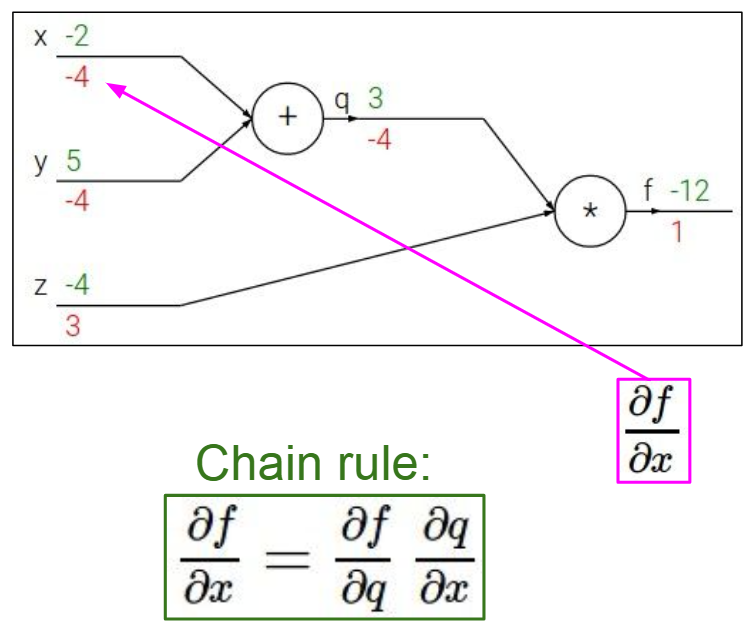
\includegraphics[scale=.5]{chap3/image/backpropagation.png}
%    \end{center}
%    \caption{Backpropagation}
%    
%    \end{figure}
%\end{center}
%\begin{itemize}
%	\item $\frac{\partial f}{\partial z} = \frac{\partial f}{\partial f} \frac{\partial f}{\partial z} = 1*3 = 3$
%	\item $\frac{\partial f}{\partial q} = \frac{\partial f}{\partial f} \frac{\partial f}{\partial q} = 1*4 = 4$
%	\item $\frac{\partial f}{\partial x} = \frac{\partial f}{\partial f}\frac{\partial f}{\partial q} \frac{\partial q}{\partial x} = 1*4*1 = 4$
%	\item $\frac{\partial f}{\partial y} = \frac{\partial f}{\partial f}\frac{\partial f}{\partial q} \frac{\partial q}{\partial y} = 1*4*1 = 4$
%\end{itemize} \par
%Việc tìm đạo hàm riêng của các hàm $f$ theo từng biến, nói cách khác là tìm sự thay đổi của biến khi đầu ra thay đổi, làm như vậy được gọi là truyền ngược (backpropagation).

\section{Hàm mất mát và Cross-entropy}
\subsection{One-hot encoding}
One-hot encoding là biến mỗi nhãn thành một vector có kích thước bằng với tập nhãn và vị trí nhãn sẽ bằng 1 còn các vị trí còn lại sẽ bằng 0. One-hot encoding được mô tả ở Hình \ref{fig:onehot}. Số lớp cần phần loại gồm: red, yellow, green, blue; các nhãn sẽ được biểu diễn lại như bảng bên; với cột là tập nhãn, dòng là dữ liệu được biểu diễn dưới dạng one-hot encoding.
\begin{figure}[H]
\begin{center}
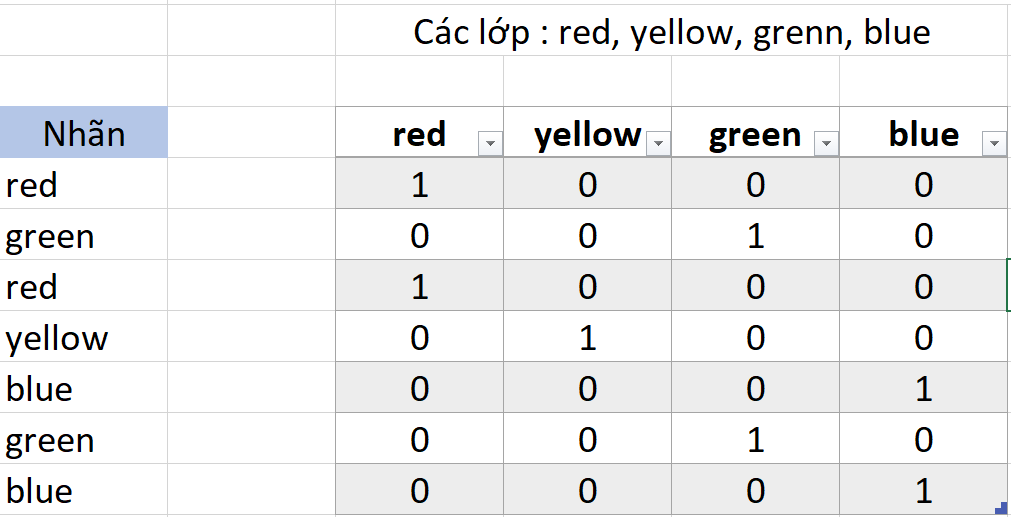
\includegraphics[scale=0.75]{chap3/image/onehot.png}

\caption{ Ví dụ one-hot encoding}
\label{fig:onehot}
\end{center}
\end{figure}
\subsection{Hàm mất mát}
Hàm mất mát hay còn gọi là \textit{loss function}, là sự chêch lệch, khác biệt giữa đầu ra dự đoán và đầu ra thực tế, có chức năng là đo độ chính xác của đầu ra dự đoán, thường được ký hiệu là $J$. Giả sử ta cần ánh xạ: $\textbf{X}\to \textbf{Y}$,  trong đó \textbf{X} là tập các vấn đề và Y là tập các lời giải tương ứng cho vấn đề đó thì ta cần xây dựng. Ta cần xây dựng hàm sao cho $\widehat{\textbf{Y}}$ =$ f(\textbf{X},\textbf{W}) \approx \textbf{Y}$. Như vậy hàm mất mát là độ chênh lệch, sự khác biệt giữa \textbf{$\widehat{\textbf{Y}}$} và $\textbf{Y}$. Nếu như giá trị mất mát càng lớn thì điều đó có nghĩa rằng đầu ra dự đoán càng sai, các tham số truyền vào chưa chính xác vì thế chúng ta cần điều chỉnh tham số sao cho hàm \textbf{$\widehat{\textbf{Y}}$} càng gần $\textbf{Y}$ càng tốt. Có nghĩa rằng chúng ta cần tìm: $\textbf{W}$=$\arg\min_{\textbf{W}} J$.\par
Trong nhiều bài toán, các mô hình tham số được định nghĩa như một phân phối $p(\textbf{y}|\textbf{x},\textbf{W})$ và sử dụng nguyên lý Maximum-Likelihood, có nghĩa là chúng ta sử dụng cross-entropy giữa $\widehat{\textbf{y}}$ và $\textbf{y}$ như là hàm mất mát. 

\subsection{Cross-entropy}
\textit{Cross entropy} là một đại lượng phản ánh mức độ khác biệt giữa hai phân phối xắc xuất. Sự khác biệt giữa phân bố $p$ và $q$ càng lớn, thì cross-entropy của $p$ đối với $q$ sẽ càng lớn hơn entropy của p.\par 
Cross entropy giữa hai vector phân phối \textbf{p} và \textbf{q} được định nghĩa là:
\begin{equation}
\label{eqn:cross1}
H(\textbf{p},\textbf{q}) = \textbf{E}_\textbf{p}[-\log(\textbf{q})]
\end{equation}\par
	Với $\textbf{p},\textbf{q} $ là rời rạc, công thức \ref{eqn:cross1} được viết dưới dạng:
\begin{equation}
\label{eqn:cross2}
H(\textbf{p}, \textbf{q}) =-\sum_{i=1}^C p_i \log q_i 
\end{equation}\par

\textbf{Chú ý}: Hàm cross entropy không có tính đối xứng $H(\textbf{p}, \textbf{q}) \neq H(\textbf{q}, \textbf{p})$. Theo công thức \ref{eqn:cross1} và \ref{eqn:cross2} chúng ta có thể thấy giá trị của $\textbf{q}$ không thể nhận giá trị là 0. Vì thể khi sử dụng cross entropy trong các bài toán học có giám sát, chúng ta phải để $\textbf{p}$ là đầu ra thực tế vì chỉ có vị trí nhãn là được đánh dấu 1, các vị trí còn lại được đánh dấu 0 (sử dụng one-hot encoding), $\textbf{q}$ là đầu ra dự đoán vì không có xắc suất nào bằng 0 tuyệt đối cả.

\subsection{Xây dựng hàm mất mát}
Giả sử số lớp chúng ta cần phân loại là $C$, xét một cặp dữ liệu $(\textbf{x}_i,\textbf{y}_i)$ với $\textbf{y}_i$ là dạng one-hot tại đầu ra thực tế thứ $i$ và đầu ra dự đoán $\widehat{\textbf{y}_i} = softmax(\textbf{a}^{(L)}_i\textbf{W}^{(L)T}_i)$. Như đã trình bày ở phần \ref{sec:softmax}, giá trị $\widehat{\textbf{y}_{ij}}$\textit{ với j=1,...,C} thể hiện xắc suất để $\textbf{x}_i$ rơi vào lớp thứ $j$. Chúng ta coi  hai vector xắc suất $\widehat{\textbf{y}_{i}}$, $\textbf{y}_i$ lần lượt là $\textbf{q},\textbf{p}$ ở trong biểu thức \ref{eqn:cross2} do đó \textit{giá trị mất mát} được tính như sau:
\begin{equation}
\label{eq:cost1}
\begin{split}
J_i(\textbf{W}) = J_i(\textbf{W};\textbf{x}_i,\textbf{y}_i) &=-\sum_{j=1}^C y_{ij} \log \widehat{y}_{ij}	\\
&= -\sum_{j = 1}^C y_{ij}\log\left(\frac{\exp(\textbf{a}^{(L-1)}_i\textbf{w}^{(L)T}_{ij})}{\sum_{k=1}^C \exp(\textbf{a}^{(L-1)}_{i}\textbf{w}^{(L)T}_{ik})}\right)\\
&= -\sum_{j=1}^C\left(y_{ji} \textbf{a}^{(L-1)}_i\textbf{w}^{(L)T}_{ij}\log\left(\sum_{k=1}^C \exp(\textbf{a}^{(L-1)}_i\textbf{w}^{(L)T}_{ik})\right)\right) \\
&= -\sum_{j=1}^C y_{ji} \textbf{a}^{(L-1)}_i\textbf{w}^{(L)T}_{ij} + \log\left(\sum_{k=1}^C \exp(\textbf{a}^{(L-1)}_i\textbf{w}^{(L)T}_{ik})\right) 
\end{split}
\end{equation}
với  $y_{ij}, \widehat{y}_{ij}$ lần lượt là phần tử thứ j của vector đầu ra thực tế (\textit{one-hot}) $\textbf{y}_i$ và vector đầu ra dự đoán $\widehat{\textbf{y}}_i$. \par

Khi dữ liệu là một tập hợp $(\textbf{x}_i,\textbf{y}_i)$, $i=1,2,...,N$ thì hàm mất mát cho \textit{softmax} được tính như sau
\begin{equation}
\label{eq:cost2}
J(\textbf{W};\textbf{X},\textbf{Y}) = -\frac{1}{N} \sum_{i=1}^N \left(  \sum_{j=1}^C y_{ji} \textbf{a}^{(L-1)}_i\textbf{w}^{(L)T}_{ij} + \log\left(\sum_{k=1}^C \exp(\textbf{a}^{(L-1)}_i\textbf{w}^{(L)T}_{ik})\right) \right)
\end{equation} 


\section{Back-propagation và tối ưu hàm mất mát}
\subsection{ Khái niệm}

Truyền ngược là Backpropagation, là một từ viết tắt cho "backward propagation of errors" tức là "truyền ngược của sai số", là một phương pháp phổ biến để \textit{huấn luyện} các mạng thần kinh nhân tạo được sử dụng \textit{kết hợp} với một \textit{phương pháp tối ưu hóa} như gradient descent, momentum, nesterov accelerated gradient, adam. Nhìn chung các phương pháp này tính toán gradient của hàm tổn thất với tất cả các trọng số có liên quan trong mạng nơ-ron đó và sử dụng nó để cập nhật các trọng số, để cực tiểu hóa hàm tổn thất. Tùy theo mỗi phương pháp sẽ có các cách cập nhật trọng số khác nhau.
\subsection{Thuật toán}
\begin{algorithm}[H]
\caption{Back-propagation}
\label{al:backward}
\begin{algorithmic}[1]
\REQUIRE Network depth, $L$
\REQUIRE $\textbf{W}^{(i)}, i \in \{1,\ldots,L \}$, ma trận trọng số của layer thứ $i$ của model
\REQUIRE $\textbf{b}^{(i)}, i \in \{1,\ldots,L \}$, bias layer thứ $i$ của model	
\REQUIRE $\textbf{X}, \textbf{x}_i, i \in \{1,\ldots,n \} $, tập dữ liệu đầu vào với $n$ là số lượng dữ liệu
\REQUIRE $\textbf{Y}$, tập đầu ra tương ứng dạng one-hot; $\textbf{y}_i, i\in \{1,\ldots,N\}$ đầu ra tương ứng với $x_i$

\FOR {$i=1;i\le N;i=i+1 $}
\STATE $\widehat{\textbf{y}} = \textbf{a}^{(l)}= f(\textbf{x}_{i},\textbf{W}_{i},\textbf{b}_{i})$

\STATE	$\textbf{e}^{(L)} = \frac{\partial J(\widehat{\textbf{W}}}{\partial \textbf{z}^{(L)}}$

\STATE $\frac{\partial J(\textbf{W})}{\partial \textbf{w}^{L}_j} = \textbf{e}^{(L)} \frac{\partial \textbf{z}^{(L)}}{\partial \textbf{w}^{(L)}_j} = \textbf{a}^{(L-1)}_{j}\textbf{e}^{(L)}$ , \textit{với mỗi $j$; $j =1,\ldots, m;$} m là số units trong layer L \\
	\FOR {$k=L-1;k \ge 1;k++$}
		\STATE $\textbf{e}^{(k)}= \textbf{e}^{(k+1)} \frac{\partial  {\textbf{z}^{(k+1)}}}{\partial \textbf{a}^{k}} \frac{\partial\textbf{a}^{k}}{\partial\textbf{z}^{k}} $
		\STATE $\frac{\partial J(\textbf{W})}{\partial \textbf{w}^{k}_j}  =\textbf{e}^{(k)} \frac{\partial \textbf{z}^{(k)}}{\partial \textbf{w}^{(k)}_j} = \textbf{a}^{(k-1)}_{j}\textbf{e}^{(k)}$,  \textit{với mỗi $j$; $j =1,\ldots, m;$} m là số units trong layer $k$ \\
		
	\ENDFOR
	\FOR {$k=L;k \ge 1;k++$} % khong cho vao phong for tren duoc do việc cập nhật có liên quan đến w
	\STATE 	\textit{cập nhật $\textbf{w}^{(k)}_j$ theo gradient $\frac{\partial J(\textbf{W})}{\partial \textbf{w}^{k}_j} $ bằng một trong các cách tối ưu như: gradient descent, adam, momentum,... với mỗi $j$; $j =1,\ldots, m$; $m$ là số units trong layer $k$}
	
	\ENDFOR
\ENDFOR
\end{algorithmic}
\end{algorithm}


\subsection{Ví dụ}
Tiếp tục ví dụ với cấu trúc mạng nơ-ron như Hình \ref{fig:baitoan}, xét một cặp dữ liệu $(\textbf{x}_i,\textbf{y}_i)$ với $\textbf{y}_i$ là dạng \textit{one-hot} tại đầu ra thực tế thứ $i$. Vì ta hiện ta chỉ xét một cặp dữ liệu vì thế tôi xin được lược bỏ chỉ số $i$ tại các công thức dưới đây. Theo như ta tính bằng \textit{feedforward }chúng ta đã có: 


\begin{itemize}
	\item[] $\textbf{a}^{(0)}=\textbf{x}_{1\times2}$
	\item[]  $\textbf{z}^{(1)}_{1 \times 3}=\textbf{a}\textbf{W}^{(1)T}_{2{\times}3}$
	\item[] $\textbf{a}^{(1)}_{1 \times 3}=\max(0,\textbf{z}^{(1)})$
	
	\item[] $\textbf{z}^{(2)}_{1\times 3}=\textbf{a}^{(1)}_{1 \times 3}\textbf{W}^{(2)T}_{3{{\times}}3 }$
	
	\item[] $\widehat{\textbf{y}}_{1\times 3} = \frac{\exp({\textbf{z}^{(2)}})}{\sum^{3}_{j=1}{\exp({\textbf{z}^{(2)}_j})}}$.

\end{itemize}
Để thực hiện thuật toán backpropagation có nghĩa là chúng ta đi tìm các giá trị sau: $\frac{\partial J_i(\textbf{W})}{\partial \textbf{W}^{(2)}},\frac{\partial J_i(\textbf{W})}{\partial \textbf{W}^{(1)}}$. Vì ta sử dụng hàm activation ở layer cuối là softmax vì thế ta có hàm mất mát là được biểu diễn theo biểu thức \ref{eq:cost2} với $J(\textbf{W})=\sum^{C}_{s=1} y_{s}{ \log \widehat{y}_{s}}$. Theo thuật toán ta cần tính $\frac{\partial J(\textbf{W})}{\partial \textbf{w}^{L}} $ tương đương với đi tìm $\textbf{e}^{L}$. Trước tiên ta sẽ đi tính phần tử một phần tử $j$ trong đó.

\begin{equation}
\begin{split}
e_j^{(L)} &= \frac{\partial J(\textbf{W}) }{\partial \textbf{z}_j^{(L)}} \\
&=-\sum^{C}_{s=1} y_{s}\frac{ \log \widehat{y}_{s}}{\partial \textbf{z}_j^{(L)}} \\
&=-\sum^{C}_{s=1} y_s \frac{1}{\widehat{y}_s}\frac{\partial \widehat{y}_s}{\partial \textbf{z}^L_j}\\
& = - y_{j}\frac{\sum^C_{k=1}\exp{(z^{(L)}_k)}}{\exp{(z^{(L)}_j)}} \frac{\exp(z^{(L)}_j) \sum^C_{k=1}\exp(z^{(L)}_k) - (\exp(z^{(L)}_{j}))^2}{\left(\sum^C_{k=1}\exp(z^{(L)}_k)\right)^2}\\
&~~ - \sum^C_{s\neq j} y_s \frac{1}{\widehat{y}_s}  \frac{0\sum^C_{s=1}\exp(z^{(L)}_s) - \exp(z^{(L)}_{s}\exp(z^{(L)}_{j}} {\left(\sum^C_{k=1}\exp(z^{(L)}_k)\right)^2}\\
&= -y_{j}\left(1-\frac{\exp(z^{(L)}_j)}{\sum^C_{k=1}\exp(z^{(L)}_k)}\right) - \sum^C_{s\neq j} y_s \frac{1}{\widehat{y}_s}\frac{\left(-\exp(z^{(L)}_{s})\exp(z^{(L)}_{j})\right)} {\left(\sum^C_{k=1}\exp(z^{(L)}_k)\right)^2} \\
& = -y_{j} \left( 1-\widehat{y}_j \right) +  \sum^C_{s\neq j}y_s \frac{1}{\widehat{y}_s}	(\widehat{y}_s	\widehat{y}_j)\\
& = \widehat{y}_j\left(\sum_{s=1}^C   y_s\right) -y_{j}\\
& = \widehat{y}_j - y_j ~~~~~~\textit{do đầu ra thực tế dạng one-hot nên tổng của nó luôn bằng 1}
\end{split}
\end{equation}
Do đó ta có
\begin{equation}
\label{eq:back_gra1}
\begin{split}
\textbf{e}^{L} & = \widehat{\textbf{y}} - \textbf{y}\\
\frac{\partial J(\textbf{W})}{\partial \textbf{W}^{L}}& = \textbf{a}^{L-1}[e_1,e_2,\ldots,e_C]=\textbf{a}^{L-1}\textbf{e}^{T}
\end{split}
\end{equation}
Nếu ta tính theo hàm mất mát đã được khai triển ở biểu thức \ref{eq:cost1} thì việc đạo hàm khá đơn giản.
\begin{equation}
\begin{split}
\frac{\partial J(\textbf{W})}{\partial \textbf{w}^{L}_j}  
&=\frac{\partial \left( -\sum_{j=1}^C y_{j} \textbf{a}^{(L-1)}\textbf{w}^{(L)T}_{j} + \log\left(\sum_{k=1}^C \exp(\textbf{a}^{(L-1)}_i\textbf{w}^{(L)T}_{j})\right) \right)}{\partial \textbf{w}^{(L)}_j}\\
&=-y_{j}\textbf{a}^{(L-1)} + 
\frac{\exp(\textbf{w}_j^{(L-1)T}\textbf{a}^{(L-1)})}{\sum_{k = 1}^C \exp(\textbf{w}_k^{(L-1)T}\textbf{a}^{(L-1)})}\textbf{a}^{(L-1)} \\
&= -y_{j}\textbf{a}^{(L-1)} + a^{(L)}_{j} \textbf{a}^{(L-1)}= \textbf{a}^{(L-1)} (a^{(L)}_{j} - y_{j})~ \text{với} ~a_j^{L} = \widehat{y}_j \\
&= e^{(L)}_{j}\textbf{a}^{(L-1)} ~(\text{với}~ e^{L}_{j} = a^{(L)}_{j} - y_{j})
\end{split}
\end{equation} 
Tổng quát ta có:
\begin{equation}
\frac{\partial J(\textbf{W})}{\partial \textbf{W}^{L}} = \textbf{a}^{L-1}[e_1,e_2,\ldots,e_C]=\textbf{a}^{L-1}\textbf{e}^{T}
\end{equation}
Chúng ta có thể thấy cách tính toán trên cũng cho kết quả với kết quả tại biểu thức \ref{eq:back_gra1}.
\section{Overfitting}
Overfitting là một hiệnn tượng không mong muốn thường gặp trong quá trình xây dựng mô hình, người xây dựng mô hình cần nắm được kỹ thuật để tránh hiện tượng này xảy ra.
\subsection{Tổng quan}
Để hiểu vấn đề này chúng ta sẽ cùng nhau xem qua ví dụ sau  Hình \ref{fig:overfitting}.
\begin{center}
 	\begin{figure}[H]
    \begin{center}
    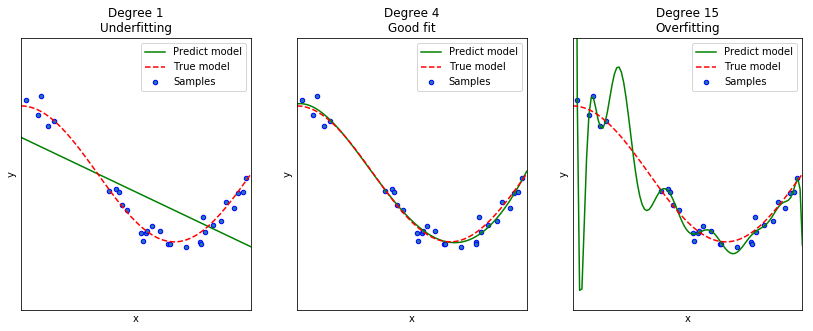
\includegraphics[scale=0.5]{chap3/image/overfitting.png}
    \end{center}
    \caption{overfitting và underfitting}
    \label{fig:overfitting}
    \end{figure}
\end{center}
Đường nét liền thể hiện \textit{mô hình dự đoán (predicted model)} , đường nét đứt thể hiện \textit{mô hình thực (true model)}, các chấm hình tròn là các điểm dữ liệu. Mô hình được xây dựng bằng hồi quy tuyến tính (\textit{linear regression}) với các feature là bậc mũ.\par
Ở hình thứ nhất chúng ta có thể thấy mô hình dự đoán là một hàm tuyến tính (bậc bằng 1) rất khác với mô hình thực, xa với các điểm dữ liệu. Hiện tượng này ta nói mô hình bị \textit{underfitting}.
Với mô hình dự đoán là đa thức bậc 4 chúng ta có thể thấy mô hình dự đoán xấp xỉ như mô hình thực (hình thứ 2). Trường hợp này ta nói mô hình phù hợp (\textit{good fit}). Ở hình thứ 3, khi ta tăng bậc đa thức lên thì mô hình dự đoán quá khớp với các điểm dữ liệu, gần như mọi điểm dữ liệu đều nằm trên mô hình. Tuy nhiên việc khớp hoàn toàn dữ liệu lại không hề tốt vì dữ liệu thường bị nhiễu và có thể khiến mô hình dự đoán bị nhiễu hơn. Trường hợp này ta nói mô hình bị\textit{ overfitting}.\\
\textbf{Một vài khái niệm về mô hình}
\begin{enumerate}
\item
\textit{Underfitting} là hiện tượng mô hình chưa được phù hợp với tập dữ liệu huấn luyện và cả các mẫu mới khi dự đoán. Nguyên nhân có thể là do mô hình chưa đủ độ phức tạp cần thiết để bao quát được tập dữ liệu.
\item   \textit{Overfitting} là hiện tượng mô hình quá khớp với \textit{tập dữ liệu huấn luyện (training set)}, việc này sẽ gây ra hậu quả vô cùng nghiêm trọng nếu tập dữ liệu huấn luyện xuất hiện nhiễu. Mô hình sẽ chỉ chú trọng vào việc xấp xỉ với tập dữ liệu huấn luyện mà quên đi mục đích ban đầu là tổng quát hóa, làm cho mô hình sẽ không thật sự tốt dối với dữ liệu nằm ngoài dữ liệu huấn luyện (dữ liệu test và dữ liệu thực tế). Overfitting xảy ra khi \textit{độ phức tạp của mô hình quá lớn} hoặc \textit{quá ít dữ liệu}.
\item \textit{Good fitting} là mô hình nằm giữa 2 mô hình chưa khớp (\textit{underfitting}) và quá khớp (\textit{overfitting}) cho ra kết quả hợp lý với cả tập dữ liệu huấn luyện và các giá trị mới, tức là nó mang được tính tổng quát như hình 1 ở giữa phía trên. Lý tưởng nhất là khớp được với nhiều dữ liệu mẫu và cả các dữ liệu mới. Tuy nhiên trên thực tế được mô hình như vậy rất hiếm.
\end{enumerate}.
\subsection{Mối liên hệ giữa overfitting và giá trị hàm mát mát}
Như tôi đã trình bày phần trên, overfitting là hiện tượng mô hình quá khớp với tập dữ liệu huấn luyện có nghĩa là giá trị của hàm mất mát trên tập dữ liệu huấn luyện (\textit{$J_{train}$}) rất nhỏ. Nhưng khi đó giá trị của hàm mất trên tập dữ liệu test (\textit{$J_{test}$}) lại tăng lên gây ra mô hình mất đi sự tổng quát. 

\begin{center}
 	\begin{figure}[H]
    \begin{center}
    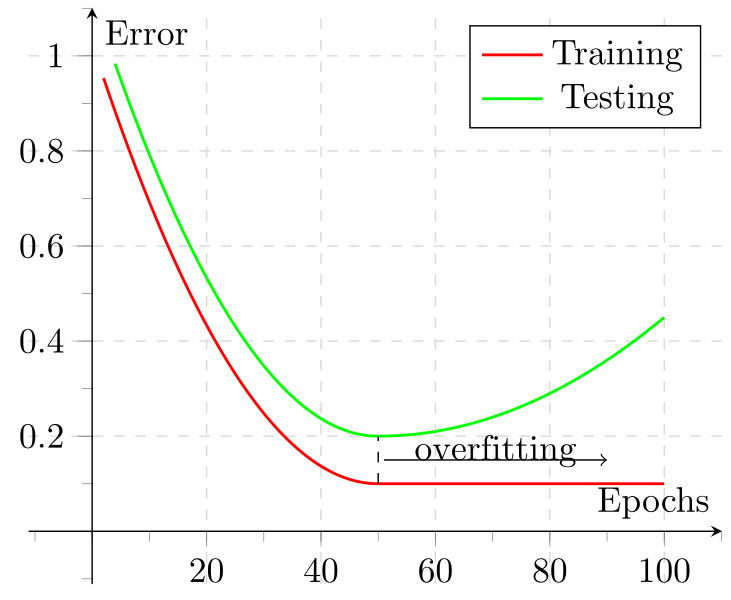
\includegraphics[scale=0.5]{chap3/image/overfittingError.png}
    \end{center}
    \caption{Overfitting xảy ra khi giá trị mất mát giữa tập train giảm còn tập test tăng}
    \label{fig:overfittingError}
    \end{figure}
\end{center}

\subsection{Regularization}

\textit{Regularization} là thay đổi mô hình một chút, chấp nhận hy sinh độ chính xác trong trainning set nhưng giảm độ phức tạp của mô hình, do đó giúp tránh được được overfitting mà vẫn giữ được tính tổng quát của mô hình.
\subsubsection{Early stopping}
Khi ta dùng một phương pháp tối ưu hàm số để giảm thiểu giá trị mất mát thì \textit{$J_{train}, J_{test}$} sẽ cùng giảm theo thời gian nhưng nếu sau một thời gian \textit{$J_{test}$} tăng lên còn \textit{$J_{train}$} tiếp tục giảm thì đó là lúc bắt đầu dẫn đến overfitting. Cách đơn giản nhất để giảm thiểu overfitting đó là dừng huấn luyện tại ngay thời điểm bắt đầu overfitting và phương pháp này được gọi là \textit{early stopping}. Nếu ta có biểu đồ về sự thay đổi giá trị mất mát của trainning và testing như Hình \ref{fig:overfittingError} thì ta có thể thấy thời điểm sử dụng early stopping là vào khoảng epochs 50.
\subsubsection{Thêm số hạng vào hàm mất mát}
Một kỹ thuật regulazation phổ biến là thêm một số hạng vào hàm mất mát như sau:
\begin{equation}
	J_{reg}(\textbf{W}) = J(\textbf{W})+ \lambda R(\textbf{W})
\end{equation}
$J(\textbf{W})$ là hàm mất mát ban đầu và cụm $ \lambda R(\textbf{W})$  mới thêm vào là số hạng chính quy hoá (hay số hạng regularization) đóng vai trò như một biện pháp phạt lỗi (penalization).\par
Trong đó, tham số chính quy hoá (\textit{regularizaton parameter}) $\lambda$ được chọn từ trước để cân bằng giữa $J(\textbf{W}) ~\text{và}~ R(\textbf{W})$. $\lambda$ càng lớn thì ta càng coi trọng $R(\textbf{W})$, ít coi trọng tham số cho hàm mất mát ban đầu hơn, dẫn tới việc các trọng số $\textbf{W}$ ít có ảnh hưởng tới mô hình hơn. Hay nói cách khác là mô hình bớt phức tạp đi giúp ta đỡ việc lỗi quá khớp.\par
$R(\textbf{W})$ thường có dạng như sau:
\begin{equation}
R(\textbf{W})= \frac{1}{p}\|\textbf{W}\|^p_p = \frac{1}{p}\sum^{n}_i |\textbf{W}|^p
\end{equation}
$p$ thường được chọn là 2 (\textit{$l_2 norm regularization$}) và 1 (\textit{$l_1 norm regularization$})\par
Phương pháp chính quy hoá này còn có tên là cắt trọng số (weight decay) vì nó khiến các hệ số trong $\textbf{W}$ không quá lớn, giúp tránh việc đầu ra phụ thuộc quá nhiều vào một đặc trưng nào đó.
\subsubsection{Drop-out}
Drop-out là một kĩ thuật Regularization để chống lại vấn đề overfitting. Cách dropout thực hiện là xoá bỏ một số unit trong các step training ứng với một giá trị xác suất $\textbf{p}$ cho trước. Các mạng mới sau khi áp dụng dropout được gọi là subsample. Thông thường xắc suất ở layer input bằng 0.8 hay ta loại bỏ khoảng 20\% số unit, ở hidden layer thì xắc suất là 0.5 có nghĩa là ta loại bỏ 50\% số unit ở layer sử dụng dropout.

\begin{center}
 	\begin{figure}[H]
    \begin{center}
    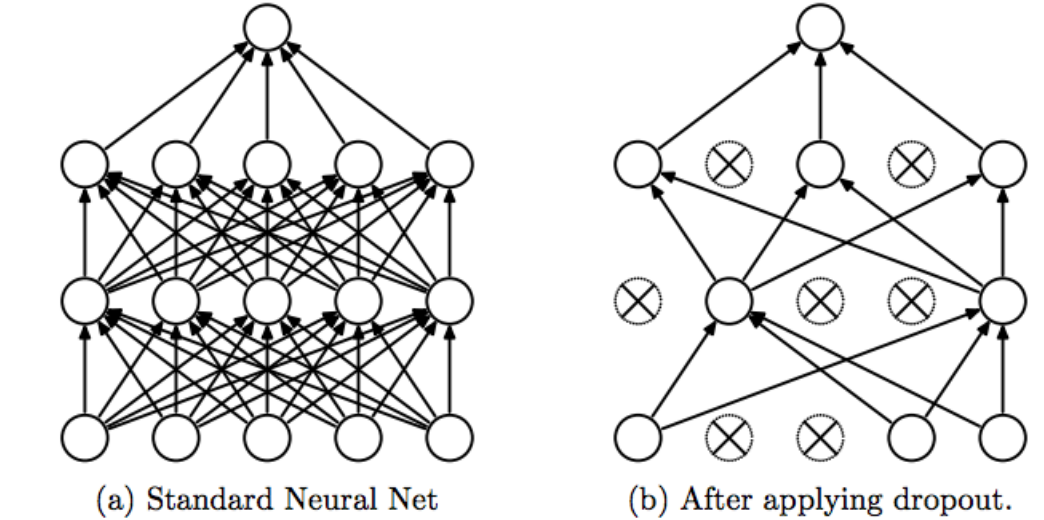
\includegraphics[scale=0.4]{chap3/image/dropout.png}
    \end{center}
    \caption{Dropout với p =0.5 và (b) là một subsample}
    \label{fig:dropout}
    \end{figure}
\end{center}

Cách hoạt động của dropout
\begin{itemize}
\item[•] Dropout được áp dụng trên một layer của mạng neural networks với một xác suất $\textbf{p}$ cho trước (có thể sử dụng nhiều Drop-Out khác nhau cho những layer khác nhau, nhưng trên 1 layer sẽ chỉ có 1 dropout)
\item[•] Tại mỗi step trong quá trình training, khi thực hiện feedforward đến layer sử dụng dropout, thay vì tính toán tất cả unit có trên layer, tại mỗi unit ta "gieo xúc xắc" với xắc suất $p$ xem unit đó được tính (active) hay không được tính (deactive). Những unit active ta tính toán bình thường còn với những unit deactive thì ta set giá trị tại unit đó bằng 0
\item[•] Trong quá trình test thì tất cả các unit đều được active và chúng ta mong muốn đầu ra của các units giống với đầu ra mong đợi trong quá trình trainning. Ví dụ đầu ra của một unit (trước khi drôput) là $\textbf{a}$, khi áp dụng dropout thì đầu ra mong đợi của unit đó sẽ là $\textbf{p}\textbf{a} + (1-\textbf{p})0$, vì unit bị deactive thì giá trị của unit đó là 0. Do đó trong quá trình test chúng ta điều chỉnh đầu ra $\textbf{a} \to \textbf{p}\textbf{a}$ để  giống với đầu ra mong đợi.
\end{itemize} \par
Thời gian test khá là quan trọng nên nếu chúng ta điều chỉnh đầu ra ở các layer áp dụng dropout thì hiệu suất test sẽ bị giảm đi. Vì thế thay vì chỉnh trong quá trình test thì chúng ta sẽ thực hiện việc này trong quá trình trainning. Ta sẽ lấy \textit{dropout mask} (vector xắc suất được khởi tạo ngẫu nhiên, tại vị trí có giá trị nhỏ hơn $p$ sẽ được giữ nguyên còn lớn hơn $p$ sẽ set lại giá trị vị trí đó là 0) chia cho $p$ trong quá trình trainning. Trường hợp này được gọi là \textit{inverted dropout}.